\section{Grådige Algoritmer}
\hrulefill

\begin{itemize}
\item Elementer af en grådig algoritme
\item Huffmann code
  \begin{itemize}
  \item Bygge en Huffman code
  \item Bevis af greedy choice
  \item Bevis af optimal delstruktur
  \end{itemize}
\end{itemize}

\newpage
\subsection{Elementerne af en grådig algoritme}
Grådige algoritmer er algoritmer der læser et problem ved altid at tage den beslutning der, lokalt, er den bedste beslutning. Grådige algoritmer, ligesom dynamisk programmering, løser problemer der udviser \textbf{optimal delstruktur}, men i modsætning til dynamisk programmering, der sørger for at tage en global optimal løsning, ved at bruge delløsninger, så tager den grådige algoritme det valg der fører til en lokal optimal løsning, hvilket i mange tilfælde også fører til den globalt optimale løsning.\\
Vi kalder den egenskab hvor en lokal optimal beslutning fører til en global optimal løsning, for \textbf{greedy choice} egenskaben.\\

\subsection{Huffman code}
Huffman code er en metode til at komprimere data på. I vores tilfælde vil vi kigge på at komprimere en streng af character tegn.\\
Hvert tegn har en bit streng der repræsenterer det tegn, f.eks. ASCII tegn er 8-bit \textbf{fixed-length code}, men det vil også sige, at hvis har en fil med 1000 tegn, så skal vi minimum bruge 8000 bits for at alle tegn med. Hvis man kun har begrænset antal tegn, kan man benytte \textbf{variable-length code}. Her giver vi tegn der optræder oftest en kortere bit længde end tegn der optræder få gange, vi sørger også for at den code vi bruger er en \textbf{prefix (free) code}, betydende at intet tegns codeword svarer til prefix af et andet tegns codeword e.g. 110 er prefix af 1101, derfor kan begge de to codewords ikke bruges.\\

\subsubsection{Bygge en Huffman code}
Algoritmen til at lave Huffman code ud fra et alfabet af tegn, går ud på at konstruere et binært træ, hvor, når man vandrer igennem træet fra roden af, så når man tager ned til venstre barn, så tilføjer man et 0, og når man tager ned mod højre barn tilføjer man 1.

 \begin{algorithm}[H]
    \caption{$N(C, i)$ with memoization}
    \begin{algorithmic}[1]
    \Function{HUFFMAN}{$C$}
    \State $n = |C|$
    \State $Q = C$ \Comment{min-prioritetskø}
    \For{$i=1$ \textbf{to} $n-1$}
    \State lav en ny knude $z$
    \State $z.left =$ EXTRACT-MIN($Q$)
    \State $z.right =$ EXTRACT-MIN($Q$)
    \State $z.freq = z.left.freq + z.right.freq$
    \State INSERT($Q, z$)
    \EndFor
    \State \textbf{return} EXTRACT-MIN($Q$) 
    \EndFunction
    \end{algorithmic}
\end{algorithm}

Algoritmen laver en prioritetskø $Q$, så tegnet med den laveste frekvens ligger først, derefter laver den en knude der forbinder de to elementer i køen med laveste frekvens og bygger træet op af.\\

Nedenunder er et eksempel på et færdigt Huffman træ med et alfabet $C$, hvor hvert tegn har frekvens $c.freq$.


\begin{center}
  $C=$
  \begin{tabular}{c|c|c|c|c|c}
  a & b & c & d & e & f\\
  \hline
  45 & 13 & 12 & 16 & 9 & 5
  \end{tabular}
\end{center}

\begin{figure}[H]  
\begin{center}
\caption{Huffman træ for $C$}
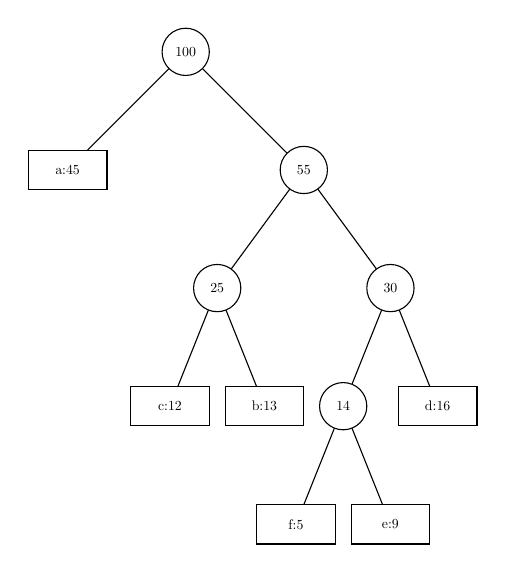
\begin{tikzpicture}[every node/.style = {shape=circle, inner sep=0pt, minimum size=1.2cm, draw, align=center, scale=0.5}, level distance=1.5cm,
          level 1/.style={sibling distance=3cm},
          level 2/.style={sibling distance=2.2cm},
          level 3/.style={sibling distance=1.2cm},
          level 4/.style={sibling distance=1.2cm}]
          \node at (0,0) {100}
          child { node[shape=rectangle, minimum height=1cm, minimum width=2cm] {a:45} }
          child { node {55} 
            child { node {25} 
                child { node[shape=rectangle, minimum height=1cm, minimum width=2cm] {c:12} }
                child { node[shape=rectangle, minimum height=1cm, minimum width=2cm] {b:13} }}
            child { node {30} 
                child { node {14} 
                    child { node[shape=rectangle, minimum height=1cm, minimum width=2cm] {f:5} }
                    child { node[shape=rectangle, minimum height=1cm, minimum width=2cm] {e:9} }}
                child { node[shape=rectangle, minimum height=1cm, minimum width=2cm] {d:16} }}};
\end{tikzpicture}
\end{center}
\end{figure}

Med fixed-length vil filstørrelsen (hvor mange bits vi skal bruge) være 8 gange så stor som antallet af tegn, hvis vi bruger ASCII. For at udregne hvor mange bits vi skal bruge med den nye prefix-code, skal vi summere produktet af tegnenes frekvens og deres dybde i træet, $d_T(c)$, som er antallet af bits i tegnets nye code. Den cost-funktion kalder $B(T)$.

$$B(T) = \sum_{c \in C} c.freq \cdot d_T(c)$$

For at bevise korrektheden af algoritmen, skal vi vise at den har greedy choice egenskaben og optimal delstruktur.

\subsubsection{Bevis af greedy choice}
Det grådige valg algoritmen tager er altid at vælge de to tegn med lavest frekvens til at være børn af en ny knude. Altså at $x,y$ har samme længde og kun skiller sig fra hinanden i den sidste bit.\\

\begin{lemma}
Lad $x, y$ være to tegn i et alfabet $C$, med laveste frekvens. Der findes en optimal prefix-code, således at koden for $x$ og $y$ har samme længde, og skiller sig kun ud i den sidste bit.\\
\end{lemma}
Altså, at træet $T$ med der indeholder det grådige valg, er optimal.\\

\begin{proof}
Vi starter med at have et træ $T$ som ikke indeholder det grådige valg, hvor $x$ og $y$ ikke er naboer. Vi ændrer så i træet indtil $x$ og $y$ er naboer, så de får samme længde og kun skiller sig ud fra hinanden i den sidste bit.\\
Lad $a, b$ være to knuder med maksimal dybde. Vi antager følgende:
\begin{itemize}
    \item $x.freq \leq y.freq$
    \item $a.freq \leq b.freq$
    \item $x.freq \leq a.freq$
    \item $y.freq \leq b.freq$
    \item $x.freq < b.freq$
\end{itemize}
Hvis $x.freq = b.freq$ så vil alle frekvenserne være ens, og ingen ændringer i træet vil kunne ændre i dens cost.\\

Første trin i beviset er at tage træet $T$ og bytte plads med $a$ og $x$, så vi får et nyt træ $T'$. Derefter tager $T'$ og bytter plads med $b$ og $y$ så vi får $T''$.

\begin{figure}[H]  
\begin{center}
\caption{Trin i rykning af træ $T \rightarrow T' \rightarrow T''$ }
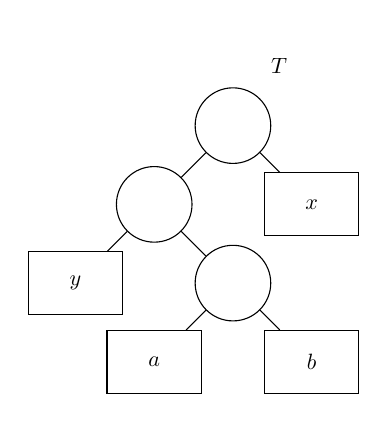
\begin{tikzpicture}[every node/.style = {shape=circle, inner sep=0pt, minimum size=1.2cm, draw, align=center, scale=0.8}, level distance=1cm,
          level 1/.style={sibling distance=2cm},
          level 2/.style={sibling distance=2cm},
          level 3/.style={sibling distance=2cm},
          level 4/.style={sibling distance=2cm}]
          \node[label= 60 :$T$] {}
          child { node {}
            child { node[shape=rectangle, minimum height=1cm, minimum width=1.5cm] {$y$}}
            child { node {}
                    child {node[shape=rectangle, minimum height=1cm, minimum width=1.5cm] {$a$} }
                    child { node[shape=rectangle, minimum height=1cm, minimum width=1.5cm] {$b$} }}}
          child { node[shape=rectangle, minimum height=1cm, minimum width=1.5cm] {$x$} };
\end{tikzpicture}
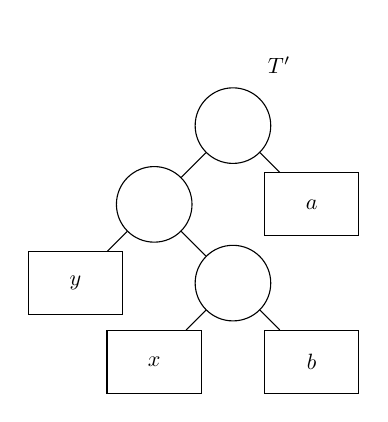
\begin{tikzpicture}[every node/.style = {shape=circle, inner sep=0pt, minimum size=1.2cm, draw, align=center, scale=0.8}, level distance=1cm,
          level 1/.style={sibling distance=2cm},
          level 2/.style={sibling distance=2cm},
          level 3/.style={sibling distance=2cm},
          level 4/.style={sibling distance=2cm}]
          \node[label= 60 :$T'$] {}
          child { node {}
            child { node[shape=rectangle, minimum height=1cm, minimum width=1.5cm] {$y$}}
            child { node {}
                    child {node[shape=rectangle, minimum height=1cm, minimum width=1.5cm] {$x$} }
                    child { node[shape=rectangle, minimum height=1cm, minimum width=1.5cm] {$b$} }}}
          child { node[shape=rectangle, minimum height=1cm, minimum width=1.5cm] {$a$} };
\end{tikzpicture}
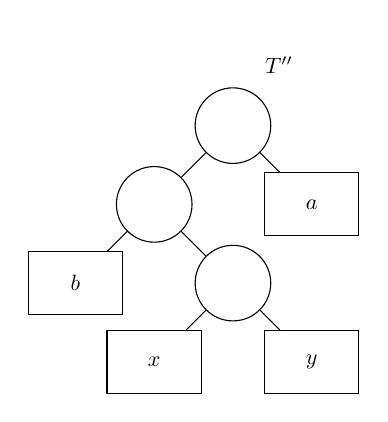
\begin{tikzpicture}[every node/.style = {shape=circle, inner sep=0pt, minimum size=1.2cm, draw, align=center, scale=0.8}, level distance=1cm,
          level 1/.style={sibling distance=2cm},
          level 2/.style={sibling distance=2cm},
          level 3/.style={sibling distance=2cm},
          level 4/.style={sibling distance=2cm}]
          \node[label= 60 :$T''$] {}
          child { node {}
            child { node[shape=rectangle, minimum height=1cm, minimum width=1.5cm] {$b$}}
            child { node {}
                    child {node[shape=rectangle, minimum height=1cm, minimum width=1.5cm] {$x$} }
                    child { node[shape=rectangle, minimum height=1cm, minimum width=1.5cm] {$y$} }}}
          child { node[shape=rectangle, minimum height=1cm, minimum width=1.5cm] {$a$} };
\end{tikzpicture}
\end{center}
\end{figure}

For at se om træet $T'$ stadig er optimalt, så skal $B(T') - B(T) \leq 0$.\\
\begin{align*}
B(T) - B(T') &= \sum_{c \in C} c.freq \cdot d_T(c) - \sum_{c \in C} c.freq \cdot d_{T'}(c)\\
            &= x.freq \cdot d_T(x) + a.freq \cdot d_T(a) - x.freq \cdot d_{T'}(x) + a.freq \cdot d_{T'}(a)\\
            &= x.freq \cdot d_T(x) + a.freq \cdot d_T(a) - x.freq \cdot d_{T}(a) + a.freq \cdot d_{T}(x)\\
            &= (a.freq - x.freq)(d_T(a) - d_T(x))
\end{align*}

Siden $x.freq \leq a.freq$ må første led være ikke negativt, og da vi ved at $a$ havde maksimal dybde i træet, må $d_T(a) - d_T(x)$ også være ikke negativt, det betyder at $0 \leq B(T) - B(T')$ og $T'$ er derfor stadig optimal. Samme argument kan bruges i $B(T') - B(T'')$, da vi nu rykker på $y$ og $b$.\\

Ergo er træet $T''$, der indeholder det grådige valg, hvor $x,y$ er naboer, optimalt.
\end{proof}

\subsubsection{Bevis af optimal delstruktur}

\begin{lemma}
Lad $x,y \in C$ være tegn med minimal frekvens. Lad $C'$ være et nyt alfabet hvor $x, y$ er fjernet og erstattet af $z$, således at $C' = C - \{x,y\} \cup \{z\}$, og hvor $z.freq = x.freq + y.freq$.\\ Lad $T$ være et træ for en optimal prefix-code for $C$, så vil $T'$, der er det træ hvor $x,y$ er fjernet, være en optimal prefix code for $C'$.\\
\end{lemma}
Altså, hvis $T$ er et optimalt træ for $C$, så må $T'$, der er et deltræ af $T$, også være optimalt for $C'$, som er et delalfabet af $C$. Ergo udvises der optimal delstruktur.\\

\begin{proof}
Træet $T'$ har cost $B(T') = B(T) - x.freq - y.freq$, siden det er det samme træ som $T$, bare hvor værdien $z.freq = x.freq + y.freq$ ligger et lag højere, så $d_T(z) = y.freq - 1 = x.freq - 1$.\\

Vi vil nu bevise at deltræet $T'$ kun er optimalt, hvis $T$ også er optimal. Vi vil bevise det med en modstrid. Vi antager at $T'$ stadig er det optimale træ for $C'$ og $T$ ikke er det optimale træ for $C$, men at der findes et træ $T''$ som er optimal for $C$, så der gælder $B(T'') < B(T)$.\\

Vi laver nu et træ $T'''$ ud fra $T''$, som er et træ for $C'$, altså hvor vi fjerner $x,y$. Hvis vi nu regner på prisen af vores deltræer, har vi
\begin{align*}
    B(T''') &= B(T'') - x.freq - y.freq\\
    &< B(T) - x.freq - y.freq\\
    &= B(T')
\end{align*}

$B(T''') < B(T')$ er en modstrid, da vi antog at $T'$ var det optimale træ for $C'$. Derfor må det optimale træ for $C'$ være et deltræ af det optimale træ for $C$, og derfor være en optimal delstruktur.
\end{proof}

\begin{proof}
Vi har nu bevist korrektheden af Huffman codes ved at bevise at den udviser de to egenskaber: Greedy choice property og optimal delstruktur.
\end{proof}

\begin{figure}[H]  
  \begin{center}
    \caption{Optimal delstruktur: Billede modstriden, at $T$ ikke er optimal for $C$ når $T'$ er optimal for $C'$}
    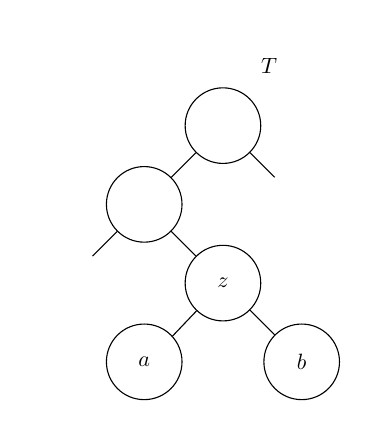
\begin{tikzpicture}[every node/.style = {shape=circle, inner sep=0pt, minimum size=1.2cm, draw, align=center, scale=0.8}, level distance=1cm,
      level 1/.style={sibling distance=2cm},
      level 2/.style={sibling distance=2cm},
      level 3/.style={sibling distance=2cm},
      level 4/.style={sibling distance=2cm}]
      \node[label= 60 :$T$] {}
      child { node {}
        child { node[draw=none] {}}
        child { node {$z$}
          child { node {$a$} }
          child { node {$b$} }}}
      child { node[draw=none] {} };
    \end{tikzpicture}
    \begin{tikzpicture}[every node/.style = {shape=circle, inner sep=0pt, minimum size=1.2cm, draw, align=center, scale=0.8}, level distance=1cm,
      level 1/.style={sibling distance=2cm},
      level 2/.style={sibling distance=2cm},
      level 3/.style={sibling distance=2cm},
      level 4/.style={sibling distance=2cm}]
      \node[label= 60 :$T'$ optimal for $C'$] {}
      child { node {}
        child { node[draw=none] {} }
        child { node {$z$} }}
      child { node[draw=none] {} };
    \end{tikzpicture}
    \\
    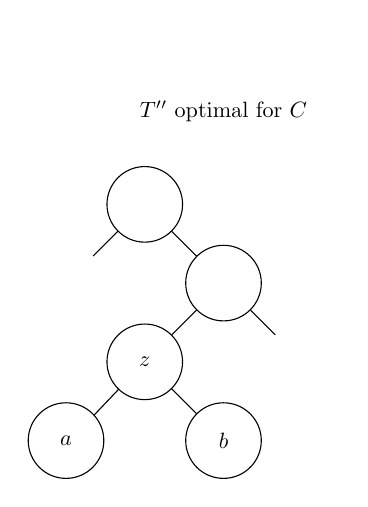
\begin{tikzpicture}[every node/.style = {shape=circle, inner sep=0pt, minimum size=1.2cm, draw, align=center, scale=0.8}, level distance=1cm,
      level 1/.style={sibling distance=2cm},
      level 2/.style={sibling distance=2cm},
      level 3/.style={sibling distance=2cm},
      level 4/.style={sibling distance=2cm}]
      \node[label= 60 :$T''$ optimal for $C$] {}
      child { node[draw=none] {}}
      child { node {}
        child { node {$z$}
          child { node {$a$} }
          child { node {$b$} }}
        child { node[draw=none] {} }};
    \end{tikzpicture}
    \begin{tikzpicture}[every node/.style = {shape=circle, inner sep=0pt, minimum size=1.2cm, draw, align=center, scale=0.8}, level distance=1cm,
      level 1/.style={sibling distance=2cm},
      level 2/.style={sibling distance=2cm},
      level 3/.style={sibling distance=2cm},
      level 4/.style={sibling distance=2cm}]
      \node[label= 60 :$T''$] {}
      child { node[draw=none] {}}
      child { node {}
        child { node {$z$}}
        child { node[draw=none] {} }};
    \end{tikzpicture}
  \end{center}
\end{figure}


%%% Local Variables:
%%% mode: latex
%%% TeX-master: "master"
%%% End:
